\documentclass[english,11pt]{beamer}

\DeclareMathOperator{\Cov}{Cov}
\DeclareMathOperator{\Var}{Var}
\DeclareMathOperator{\E}{\mathbb{E}}
\DeclareMathOperator{\Proba}{\mathbb{P}}

\newcommand{\Covb}[2]{\ensuremath{\Cov\!\left[#1,#2\right]}}
\newcommand{\Eb}[1]{\ensuremath{\E\!\left[#1\right]}}
\newcommand{\Pb}[1]{\ensuremath{\Proba\!\left[#1\right]}}
\newcommand{\Varb}[1]{\ensuremath{\Var\!\left[#1\right]}}

% norm
\newcommand{\norm}[1]{\| #1 \|}

\newcommand{\indep}{\rotatebox[origin=c]{90}{$\models$}}





\usepackage{mathptmx,amsmath,amssymb,graphicx,bibentry,bbm,babel,ragged2e}

\makeatletter

\newcommand{\noun}[1]{\textsc{#1}}
\newcommand{\jitem}[1]{\item \begin{justify} #1 \end{justify} \vfill{}}
\newcommand{\sframe}[2]{\frame{\frametitle{#1} #2}}

\newenvironment{centercolumns}{\begin{columns}[c]}{\end{columns}}
%\newenvironment{jitem}{\begin{justify}\begin{itemize}}{\end{itemize}\end{justify}}

\usetheme{Warsaw}
\setbeamertemplate{footline}[text line]{}
\setbeamercolor{structure}{fg=purple!50!blue, bg=purple!50!blue}

\setbeamersize{text margin left=15pt,text margin right=15pt}

\setbeamercovered{transparent}


\@ifundefined{showcaptionsetup}{}{%
 \PassOptionsToPackage{caption=false}{subfig}}
\usepackage{subfig}

\usepackage[utf8]{inputenc}
\usepackage[T1]{fontenc}

\usepackage{multirow}


\makeatother

\begin{document}





\title{Extracting knowledge from simulation models: trends and perspectives from the viewpoint of quantitative geography}

\author{J.~Raimbault$^{1,2,\ast}$\\
\texttt{juste.raimbault@polytechnique.edu}
}


\institute{$^{1}$Complex Systems Institute, Paris, UPS CNRS 3611 ISC-PIF\\
$^{2}$UMR CNRS 8504 G{\'e}ographie-cit{\'e}s
}


\date{CCS 2018\\\smallskip
\textit{Satellite Methods and Epistemologies of Simulation}
Thessaloniki\\\smallskip
September 26th 2018
}

\frame{\maketitle}


% Keywords : }\textit{Simulation models; Quantitative geography; Open questions; Epistemological framework}

%

% note : no multi-scale ? linked to coupling
% note : link with the applied knowledge fwk ?




\sframe{A long history of simulation in TQG}{

%The role of simulation models in the production of knowledge has significantly shifted in recent years, accompanied with a transformation of practices, including methods and tools. This presentation aims at describing these mutations from the point of view of theoretical and quantitative geography.

\centering

	%\includegraphics[width=0.52\textwidth]{figures/}
	
	\footnotesize
\textit{Source: }


}


\sframe{Current trends in (geo-)simulation and OpenMole's positioning}{

% 
%\centering
\justify

% We first survey the current trends and explicit the positioning of OpenMOLE's philosophy within these.

\cite{arribas2018geography} new geographic data science

\cite{perez2016agent} key challenges in ABM for planning: addressing complexity in a clean way, addressing multi-dimensionality, feasible trajectories, participatory planning.

Simulation models \cite{banos2013pour}: interdiscplinarity, data-driven models, exploration of models, multi-objective issues, reproducibility and reuse of models, coupling models.

\cite{banos2017knowledge} deeper knowledge

\cite{behnisch2018trends} quantifying urban growth and form, mining spatio-temporal data, geosimulation, multi-scalar approaches

}


\sframe{Citation network analysis}{

% % A citation network mapping helps situating it in the broader context of computational science.

\centering

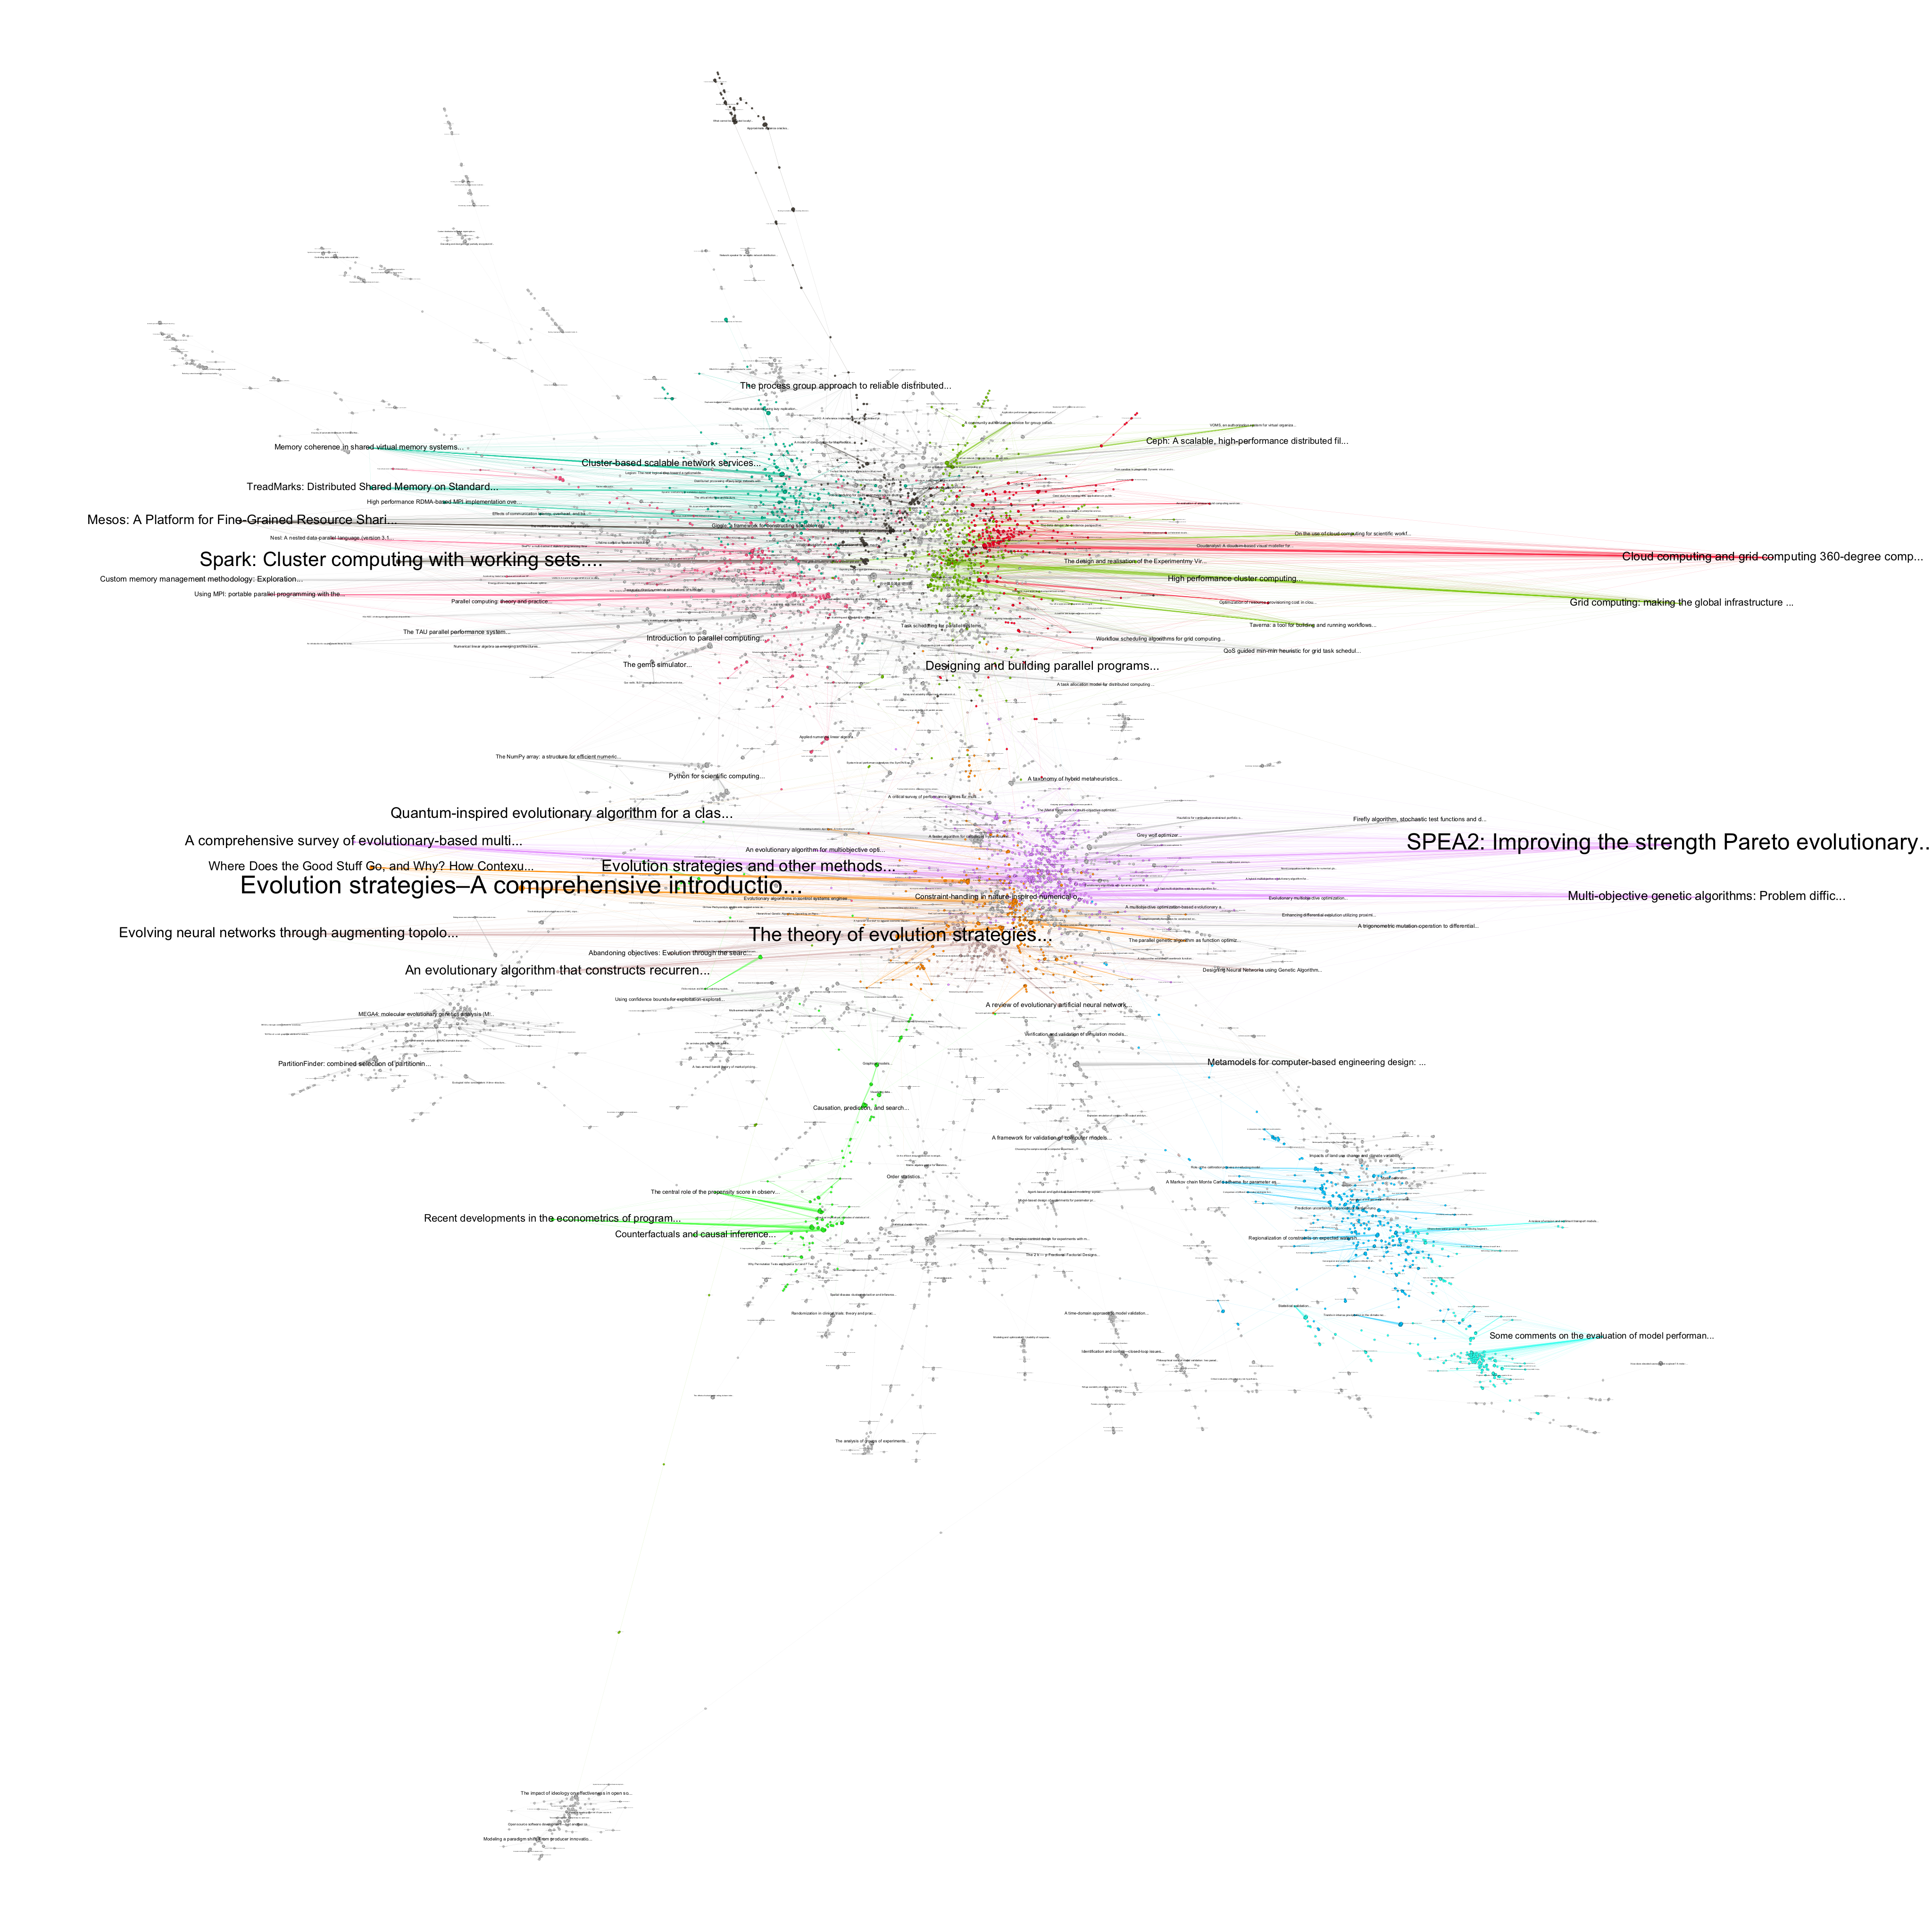
\includegraphics[width=\textwidth]{figures/citnw_sampled.png}

}


\sframe{Citation network analysis}{

\centering

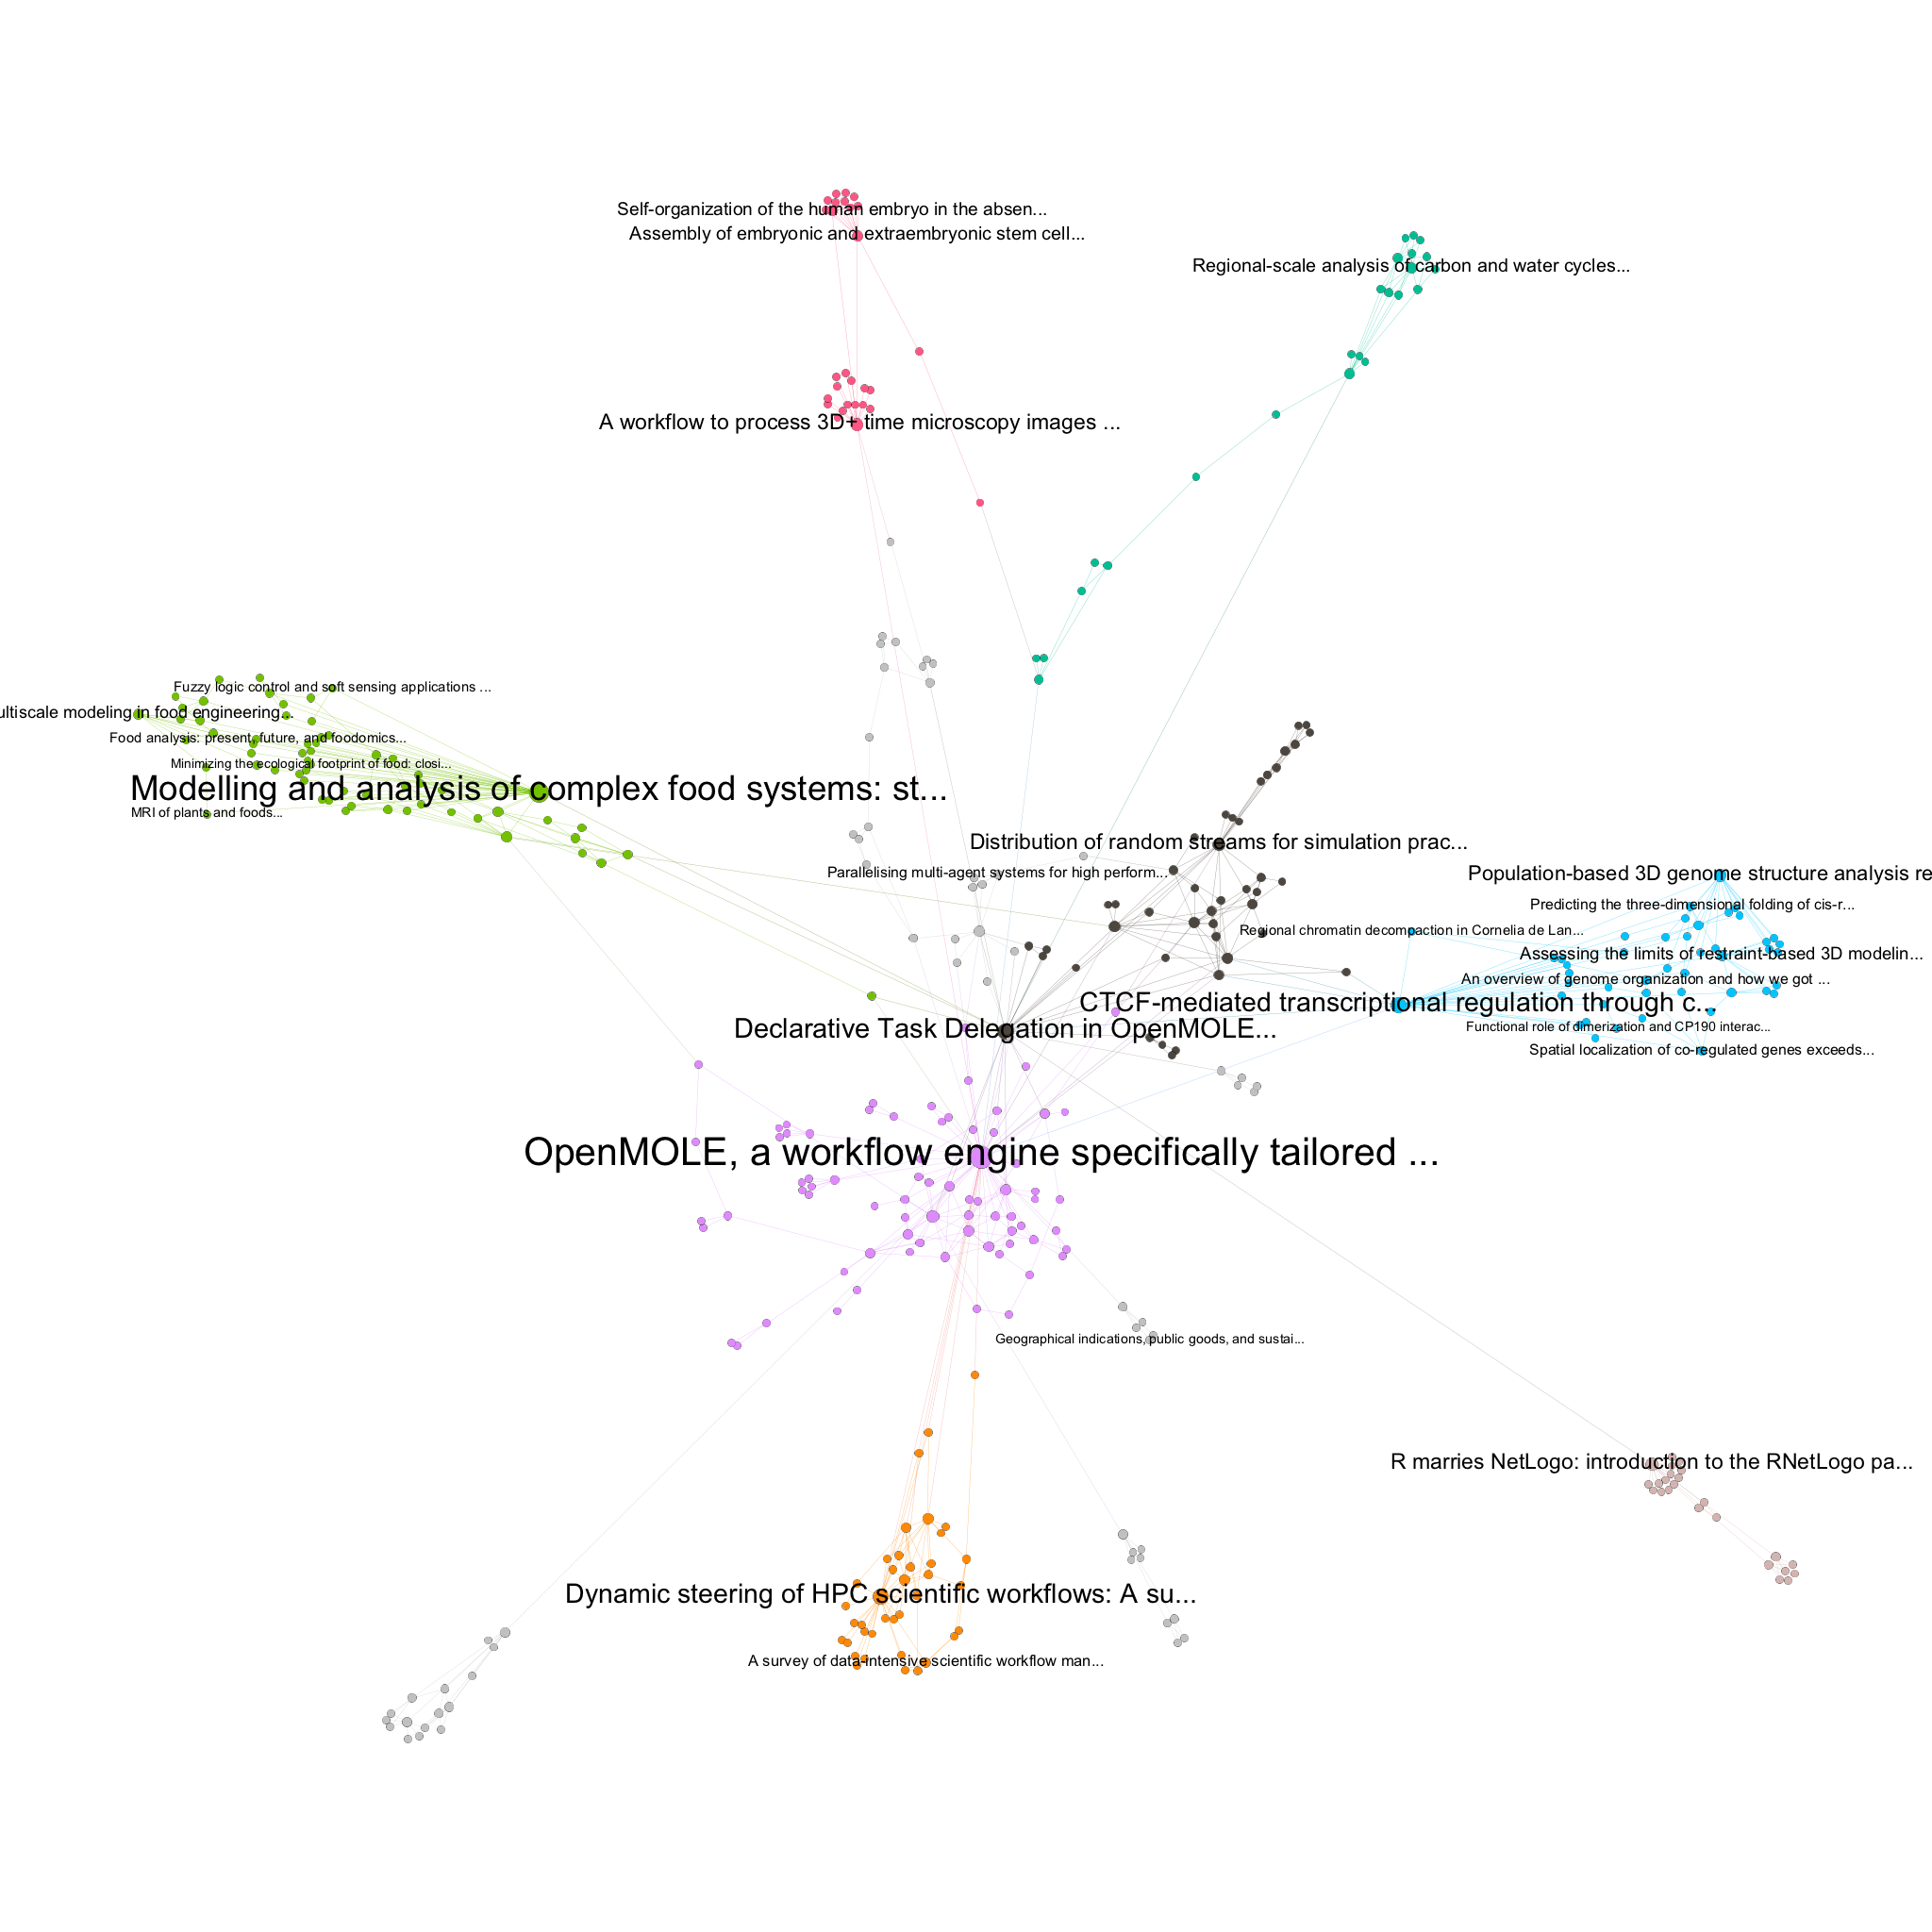
\includegraphics[width=\textwidth]{figures/oml_depth3_core.png}
}




\sframe{Perspectives and open issues for simulation in geography}{

%We then propose a grasp on some future perspectives, by detailing examples of crucial research questions on simulation models in geography that remain open, including in particular, first generic issues such as

% plan (generic + specific to spatio-temporal modeling)




}





\sframe{Dealing with overfitting}{

% (i) the development of multi-modeling techniques that explicitly account for overfitting for simulation models;

}


\sframe{Model coupling}{

% (ii) a better understanding of model coupling
% (includes multi-scale more or less)
% -> robust definition / classification of models etc



}


\sframe{Direct and inverse mapping}{

% (iii) the development of adaptative direct and inverse mapping methods;
% inverse problems / feasible space


}


\sframe{Handling stochasticity}{

% (iv) a better handling of stochasticity in ``real-world'' models;



}

\sframe{Spatio-temporal modeling issues: non-stationarity}{

%  and secondly issues which are more specific to spatio-temporal models, such as (v) the understanding of spatio-temporal non-stationarity, possibly through the intermediate of limit links between agent-based approaches and system dynamics approaches;



}


\sframe{Spatio-temporal synthetic data}{

% and (vi) methods to generate synthetic spatio-temporal data to be used for broader sensitivity analyses.

}





\sframe{An integrated view}{
	
	% graph between different open issues
	
}


\sframe{Applied perspectivism to couple modeling approaches}{

% We finally describe an epistemological framework integrating several of these issues, which applies Giere's perspectivism to the effective coupling of simulation models, and that we call ``applied perspectivism''. This framework should foster the development of integrative theories through the coupling of perspectives, and therefore of models.

% link it with knowledge framework



}






\sframe{Conclusion}{


\justify

%\vspace{-1cm}

$\rightarrow$ 

\bigskip

\footnotesize

\textbf{Related works}

Raimbault, J. (2017, December). An Applied Knowledge Framework to Study Complex Systems. In Complex Systems Design \& Management (pp. 31-45). arXiv:1706.09244.

\smallskip


Raimbault, J. (2018). Caract{\'e}risation et mod{\'e}lisation de la co-{\'e}volution des r{\'e}seaux de transport et des territoires (Doctoral dissertation, Université Paris 7 Denis Diderot). \url{https://halshs.archives-ouvertes.fr/tel-01857741}




%\smallskip

%\textbf{Open repository} at \texttt{https://github.com/JusteRaimbault/UrbanGrowth}\\\smallskip
%\textbf{Acknowledgments}: thanks to the \textit{EGI} for access to the infrastructure.


}






\sframe{Reserve slides}{

\centering

\Large

\textbf{Reserve Slides}

}



%%%%%%%%%%%%%%%%%%%%%
\begin{frame}[allowframebreaks]
\frametitle{References}
\bibliographystyle{apalike}
\bibliography{/Users/juste/ComplexSystems/CityNetwork/Biblio/Bibtex/CityNetwork,biblio}
\end{frame}
%%%%%%%%%%%%%%%%%%%%%%%%%%%%




\end{document}









